\documentclass{article}

\usepackage{enumerate}
\usepackage{amsmath}
\usepackage{amssymb}
\usepackage{amsfonts}
\usepackage{mathtools}
\usepackage{graphicx}
\usepackage{float}
\usepackage{caption}
\usepackage{subcaption}
\usepackage{color}
\usepackage{relsize}
\usepackage{algpseudocode}
\usepackage[procnames]{listings}
\usepackage[colorlinks = true, allcolors = blue]{hyperref}
\usepackage[]{units}
\usepackage{framed}
\usepackage{breqn}
\usepackage{lipsum}
\usepackage{algorithm}
\usepackage{algpseudocode}
\usepackage{fancyhdr}
\usepackage{extramarks}
\usepackage{xfrac}
\usepackage{multicol}
\usepackage{bibentry}
\usepackage{verbatim}
\nobibliography*

\def\arraystretch{1.2}

\topmargin = -0.45in
\evensidemargin = 0in
\oddsidemargin = 0in
\textwidth = 6.5in
\textheight = 9.0in
\headsep = 0.25in

\pagestyle{fancy}
\lhead{Pedro D. Bello-Maldonado}
\chead{}
\rhead{Research notes}
\lfoot{IBM Research - Sustainability}
\cfoot{\thepage}
\rfoot{\today}

\renewcommand\headrulewidth{0.4pt}
\renewcommand\footrulewidth{0.4pt}

\renewcommand{\algorithmicrequire}{\textbf{Input:}}
\renewcommand{\algorithmicensure}{\textbf{Output:}}
\renewcommand{\algorithmicforall}{\textbf{parallel for}}

\setlength{\parindent}{0pt}
\setlength{\parskip}{5pt plus 1pt minus 1pt}

\begin{document}
    \center \Large{\textbf{Energy Measurements of the Life Cycle of Foundation Models}}

    \abstract{Foundation models (FM) have become the main target of machine learning (ML) research, as they have been shown to produce human-level responses in conversational AI and image generation. Models like OpenAI's ChatGPT or Google's Bard are now mainstream tools used on a daily basis for generating code, writing essays, and many other NLP tasks. Training and deploying (i.e., running inference queries) such models requires large amounts of compute power over extended periods of time. This translates to high-energy usage, that without proper management can lead to significant amounts of carbon emissions being released to the atmosphere. This study aims to establish best practices as it relates to making FM a sustainable tool, by collecting and analyzing energy measurements of FM jobs run on cloud computing infrastructure with OpenShift.}

    \section{Introduction}
    {
        In training an AI system, the choice of hyperparameters used (i.e., learning rate, batch size, etc.) impacts the convergence of the model as well as the energy used during training. In many cases, these are competing objectives as an ideal scenario is that of a highly accurate model trained with the least amount of energy. Achieving high model accuracy is done by training over longer periods of time, increasing the number of training samples, tuning hyperparameters over several training rounds, all of which result in higher energy usage. It is very difficult to estimate how a particular hyperparameter choice affects the convergence of the model. However, a few hyperparameter choices are known to, generally, improve the convergence at the cost of more computational resources. Here we focus on the \textbf{batch size} which defines the number of training samples run \textit{together} at a time during the forward and backward pass of the training phase. The assumption here is that, a larger batch size improves the convergence of the method as the \textit{context} of the training is better understood with larger sizes, leading to faster convergence. In turn, using large batch sizes requires more memory limiting the number of samples one can use for a given hardware, and increasing the energy consumption of the system used (e.g., more GPU compute cores are activated due to increased utilization). 
    }

    \section{Methodology}
    {
        The foundation model stack (FMS) at IBM Research provides off-the-shelf tools to train foundation models on OpenShift cloud infrastructure. These are cloud-ready Python scripts to train FM models (such as the RoBERTa model used in NLP) that expose hyperparameters, such as the batch size, so users can tune the training to their liking. We treat these training scripts as \textit{black box} programs to which we attach power measuring profilers that are agnostic to the type of training being performed (see Figure~\ref{fig:architecture}).

        \begin{figure}[!h]
            \centering
            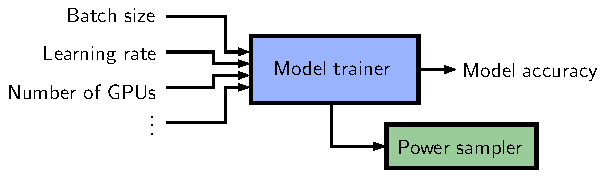
\includegraphics[width = 0.5 \textwidth]{../Figures/architecture.pdf}
            \caption{Model training and power measuring architecture}
            \label{fig:architecture}
        \end{figure}
    }

    \section{Results}
    {
        For our evaluation in this report, we focus only on the batch size and explore its impact on the model convergence and the energy (power integrated over time) consumption. The setup for this training is as follows:

        \begin{itemize}
            \item 1 compute node with: 8 GPUs, 16 CPUs, and 64 GB of memory
            \item Single POD with one PyTorch container
            \item NCCL communication enabled
        \end{itemize}

        \noindent The model is trained for exactly $N = 400000$ steps while reporting the training loss every 10 steps and the validation loss every 5000 steps. We first look at the results using the training loss as the accuracy metric. Figure~\ref{fig:unstopped_execution_training} shows the overall convergence over the duration of the training as well as the energy consumed during that training. The top row shows the horizontal axis as the number of steps, while the bottom row shows the horizontal axis as time. As expected, for the same number of steps, larger batch sizes take longer to compute, resulting in longer training jobs and higher energy consumption.

        \begin{figure}[!t]
            \centering
            \captionsetup[subfigure]{margin = {0.0in,0.0in}}
            \begin{subfigure}[b]{0.47 \textwidth}
                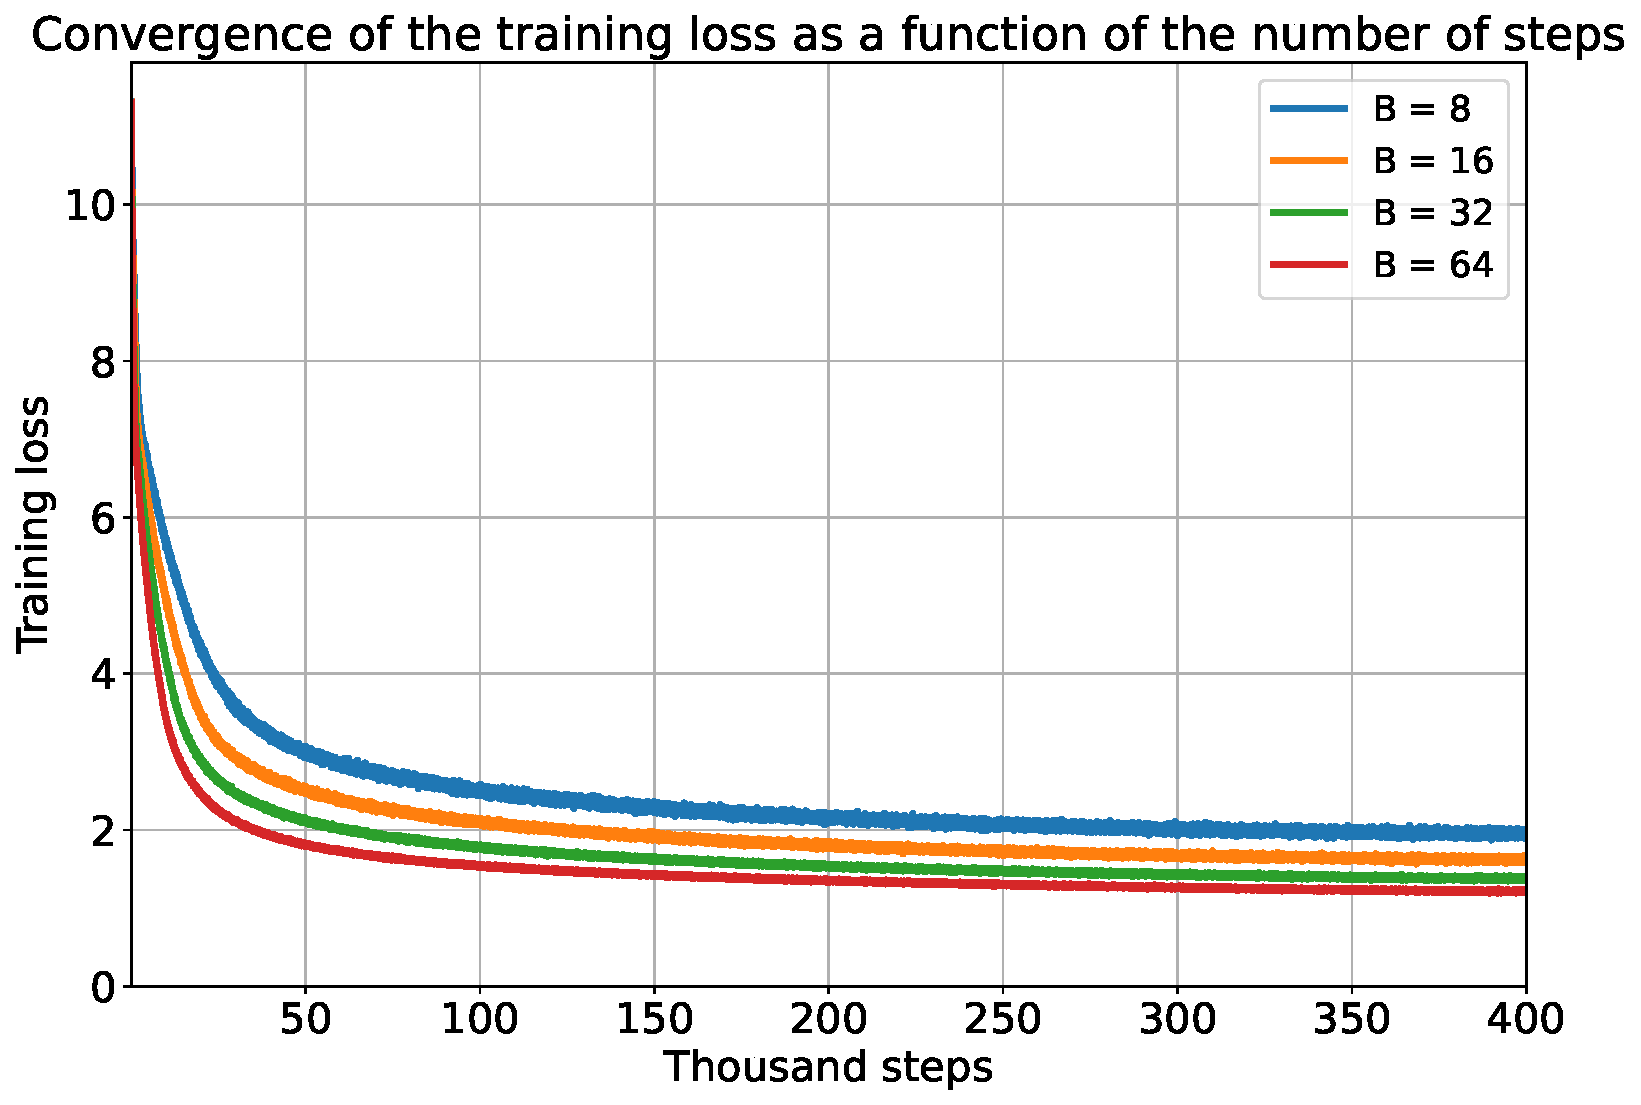
\includegraphics[trim = {0.0in 0.0in 0.0in 0.0in}, clip, width = 1.0 \textwidth]{../Figures/convergence_history_training.pdf}
                \caption{Convergence as a function of the number of steps}
                \label{fig:convergence_accuracy_training}
            \end{subfigure}
            ~
            \captionsetup[subfigure]{margin = {0.2in,0.0in}}
            \begin{subfigure}[b]{0.47 \textwidth}
                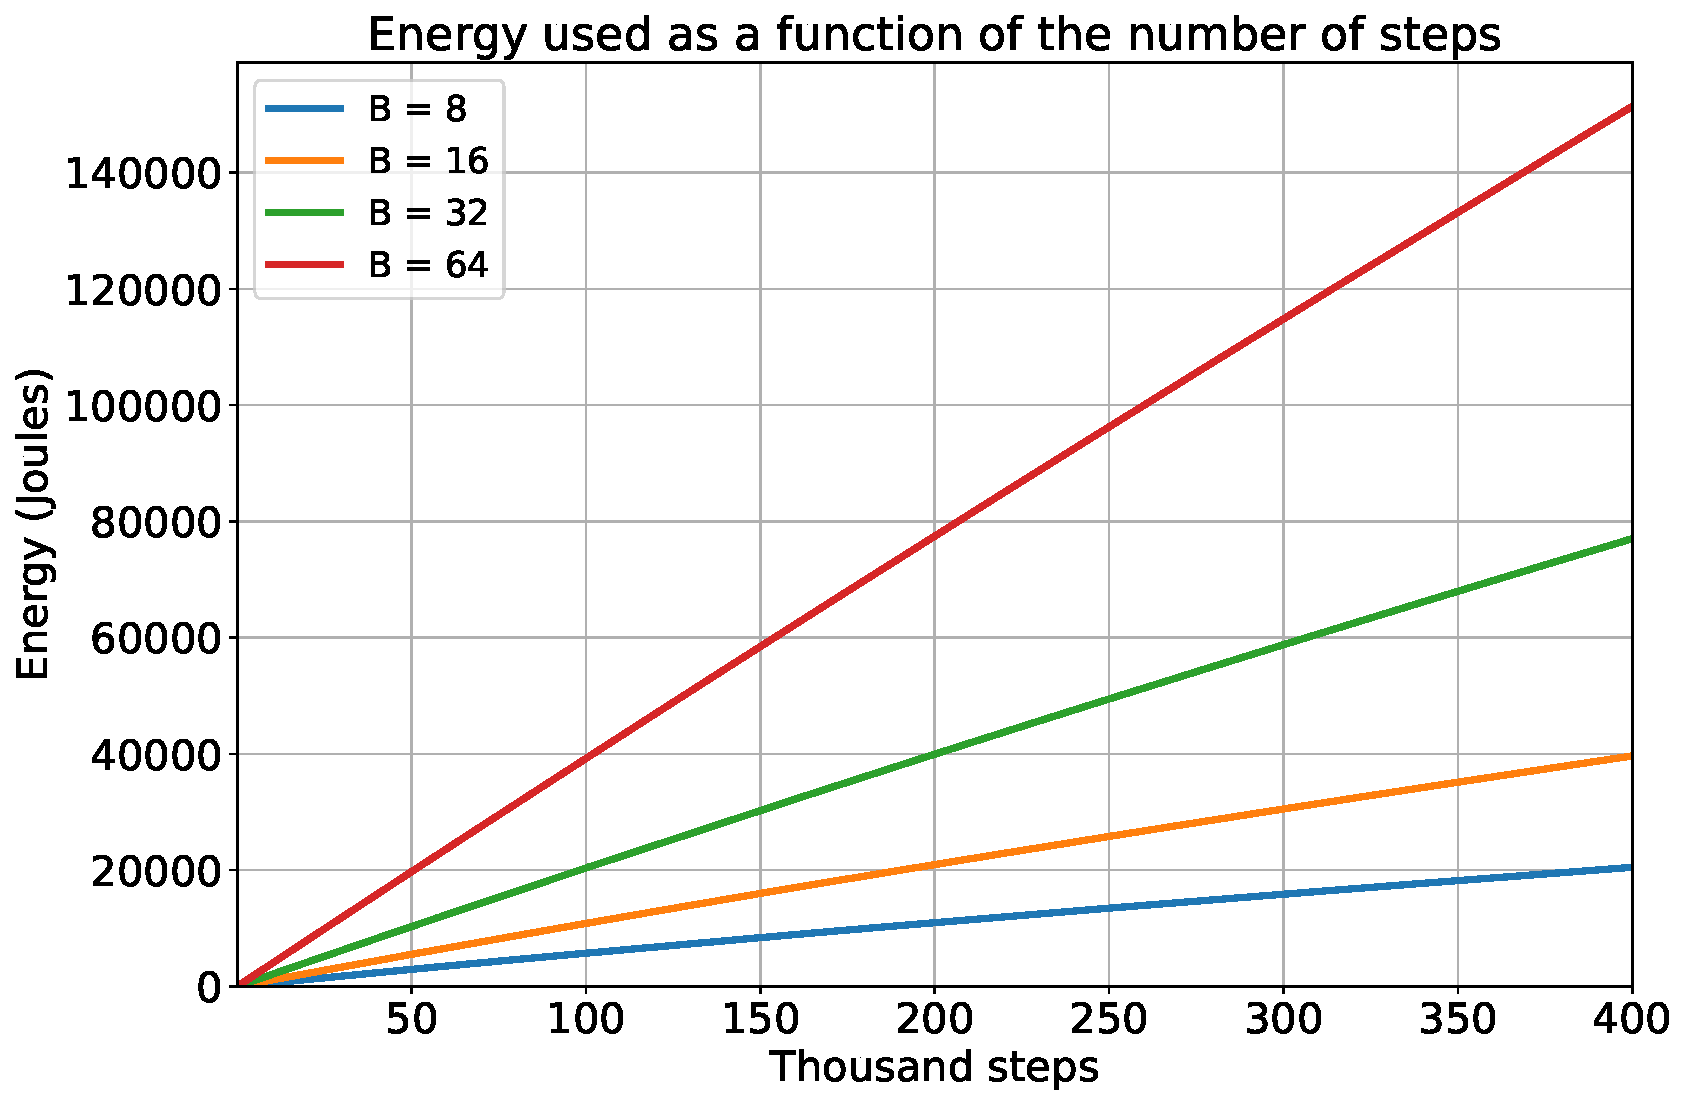
\includegraphics[trim = {0.0in 0.01in 0.0in 0.0in}, clip, width = 1.025 \textwidth]{../Figures/energy_history_training.pdf}
                \caption{Energy used as a function of the number of steps}
                \label{fig:convergence_energy_training}
            \end{subfigure}
            ~
            \captionsetup[subfigure]{margin = {0.0in,0.0in}}
            \begin{subfigure}[b]{0.47 \textwidth}
                \vspace{1.0em}
                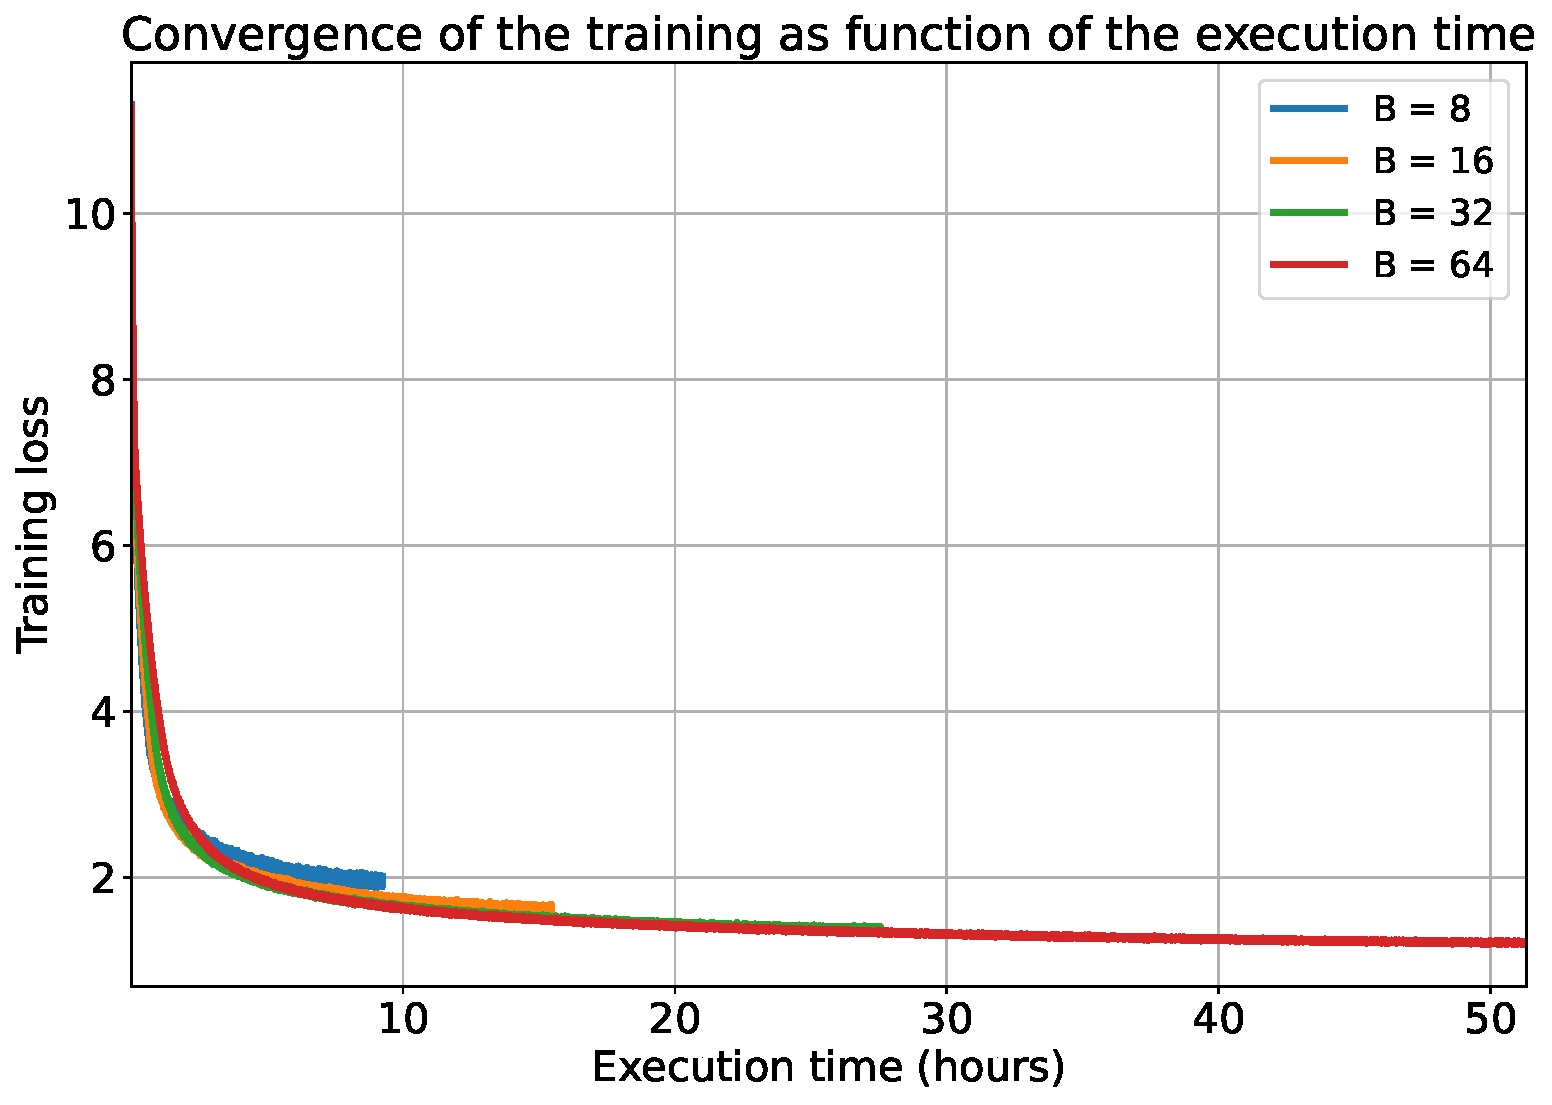
\includegraphics[trim = {0.0in 0.0in 0.0in 0.0in}, clip, width = 1.0 \textwidth]{../Figures/time_vs_accuracy_training.pdf}
                \caption{Convergence as a function of the execution time}
                \label{fig:time_vs_accuracy_training}
            \end{subfigure}
            ~
            \captionsetup[subfigure]{margin = {0.2in,0.0in}}
            \begin{subfigure}[b]{0.47 \textwidth}
                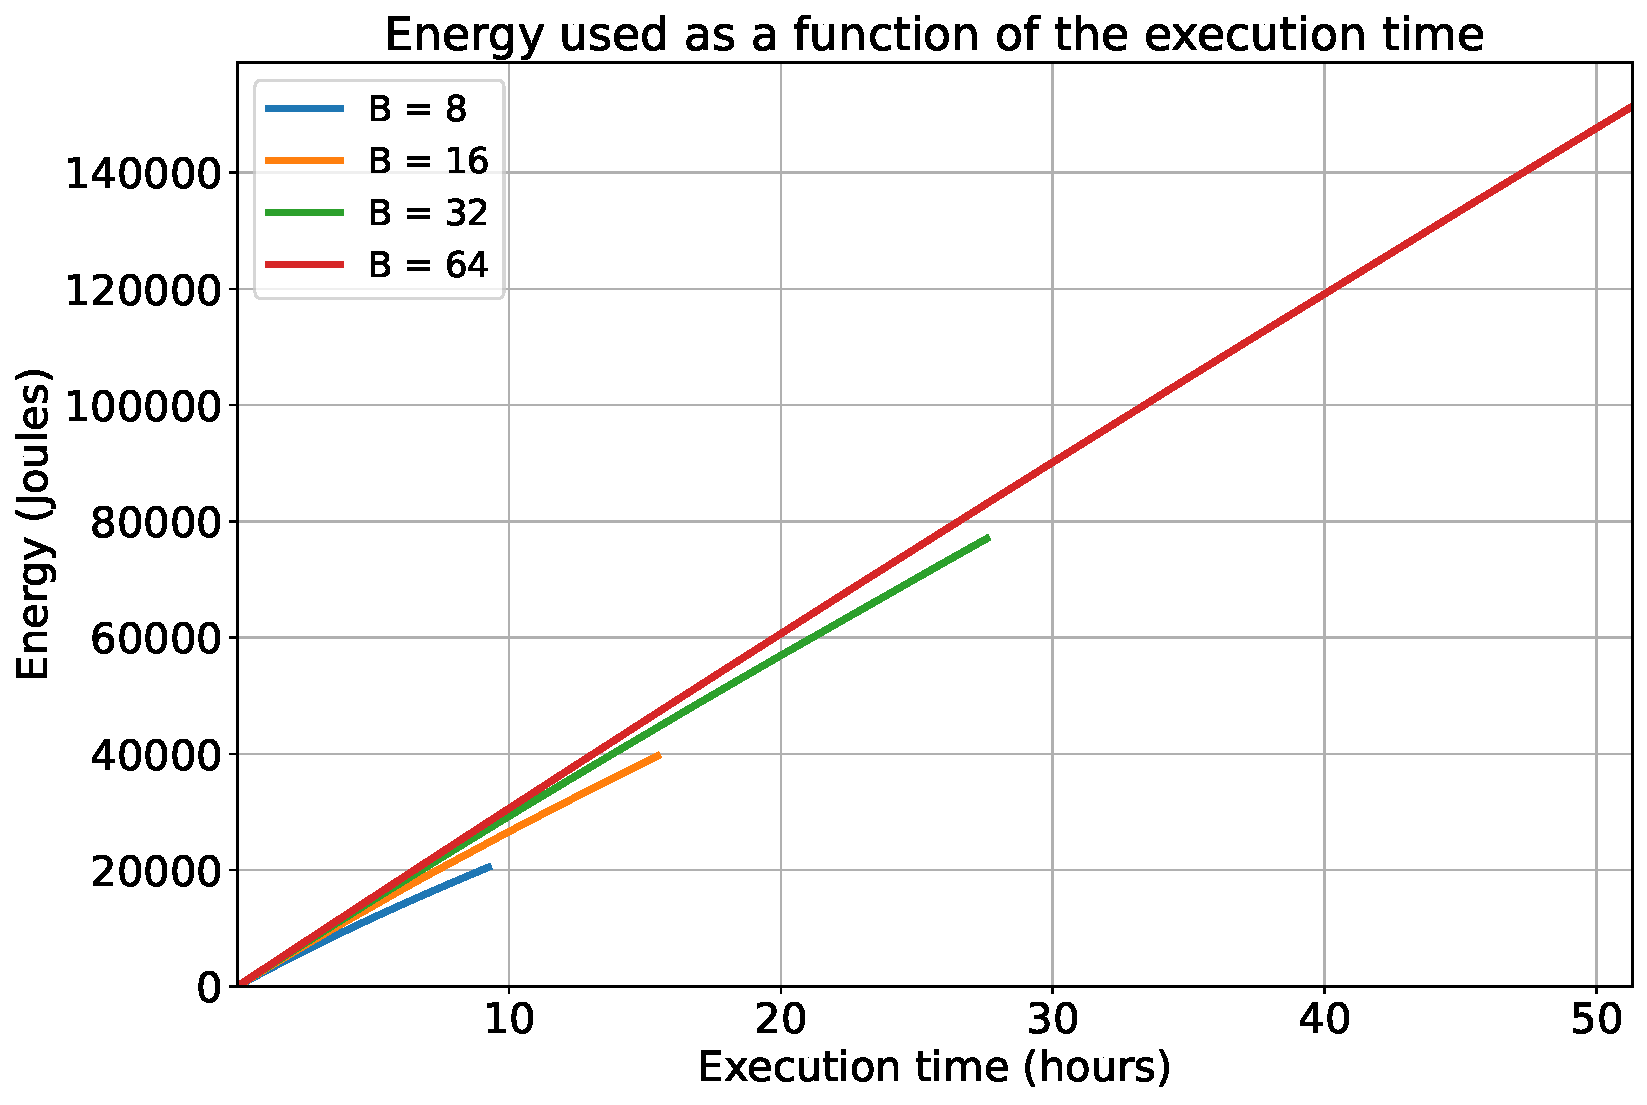
\includegraphics[trim = {0.0in 0.01in 0.0in 0.0in}, clip, width = 1.060 \textwidth]{../Figures/time_vs_energy_training.pdf}
                \caption{Energy used as a function of the execution time}
                \label{fig:time_vs_energy_training}
            \end{subfigure}
            \caption{Convergence and energy measurements over the complete unstopped execution (i.e., all $N = 400000$ training steps)}
            \label{fig:unstopped_execution_training}
        \end{figure}

        In practice, a training job is stopped once an accuracy \textit{threshold} is reached thus saving time and energy. As shown in Figure~\ref{fig:convergence_accuracy_training}, a larger batch size leads to faster convergence as shown by the larger batch sizes reaching lower training losses with fewer number of steps. However, the energy and computational cost-per-iteration (i.e., runtime) is higher with larger batch sizes making the choosing of batch size unclear. In Figure~\ref{fig:convergence_threshold_training} we look at the energy consumed by the training once the algorithm has reached a prespecified threshold.

        \begin{figure}[!t]
            \centering
            \captionsetup[subfigure]{margin = {0.2in,0.0in}}
            \begin{subfigure}[b]{0.47 \textwidth}
                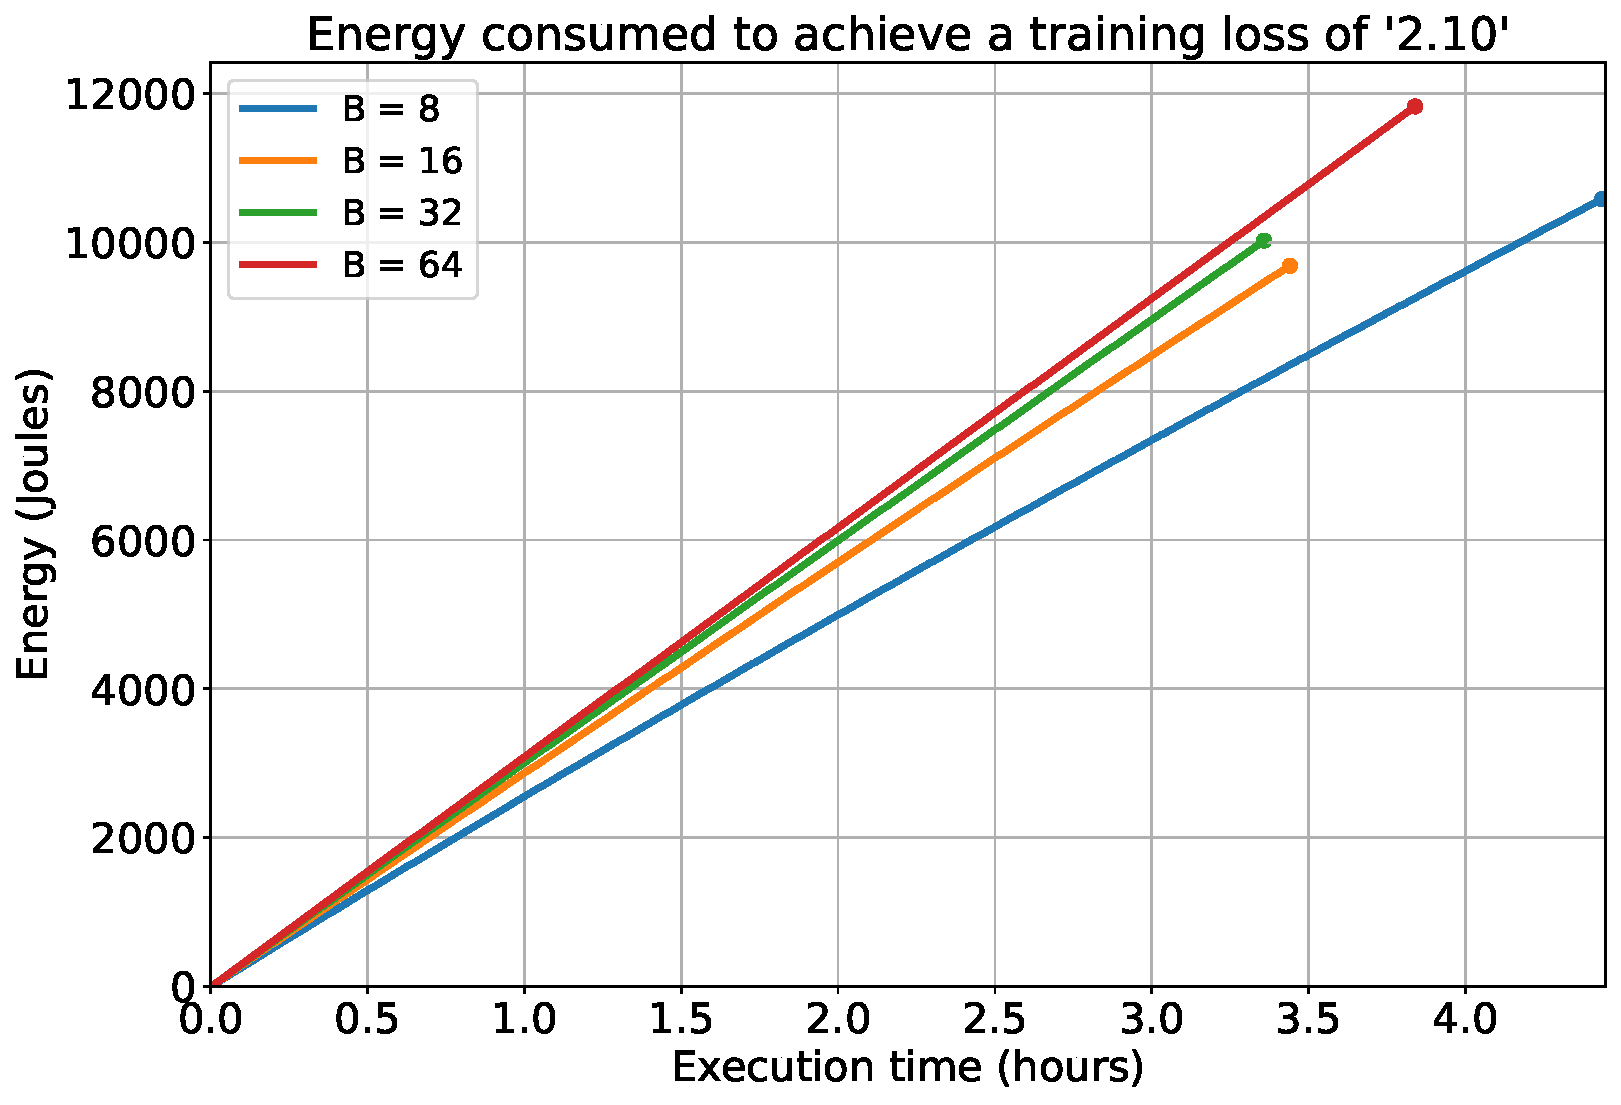
\includegraphics[trim = {0.0in 0.0in 0.0in 0.0in}, clip, width = 1.0 \textwidth]{../Figures/time_vs_energy_converged_training_210.pdf}
                \caption{Energy for converging to training loss of $2.1$}
                \label{fig:convergence_energy_training_210}
            \end{subfigure}
            ~
            \captionsetup[subfigure]{margin = {0.2in,0.0in}}
            \begin{subfigure}[b]{0.47 \textwidth}
                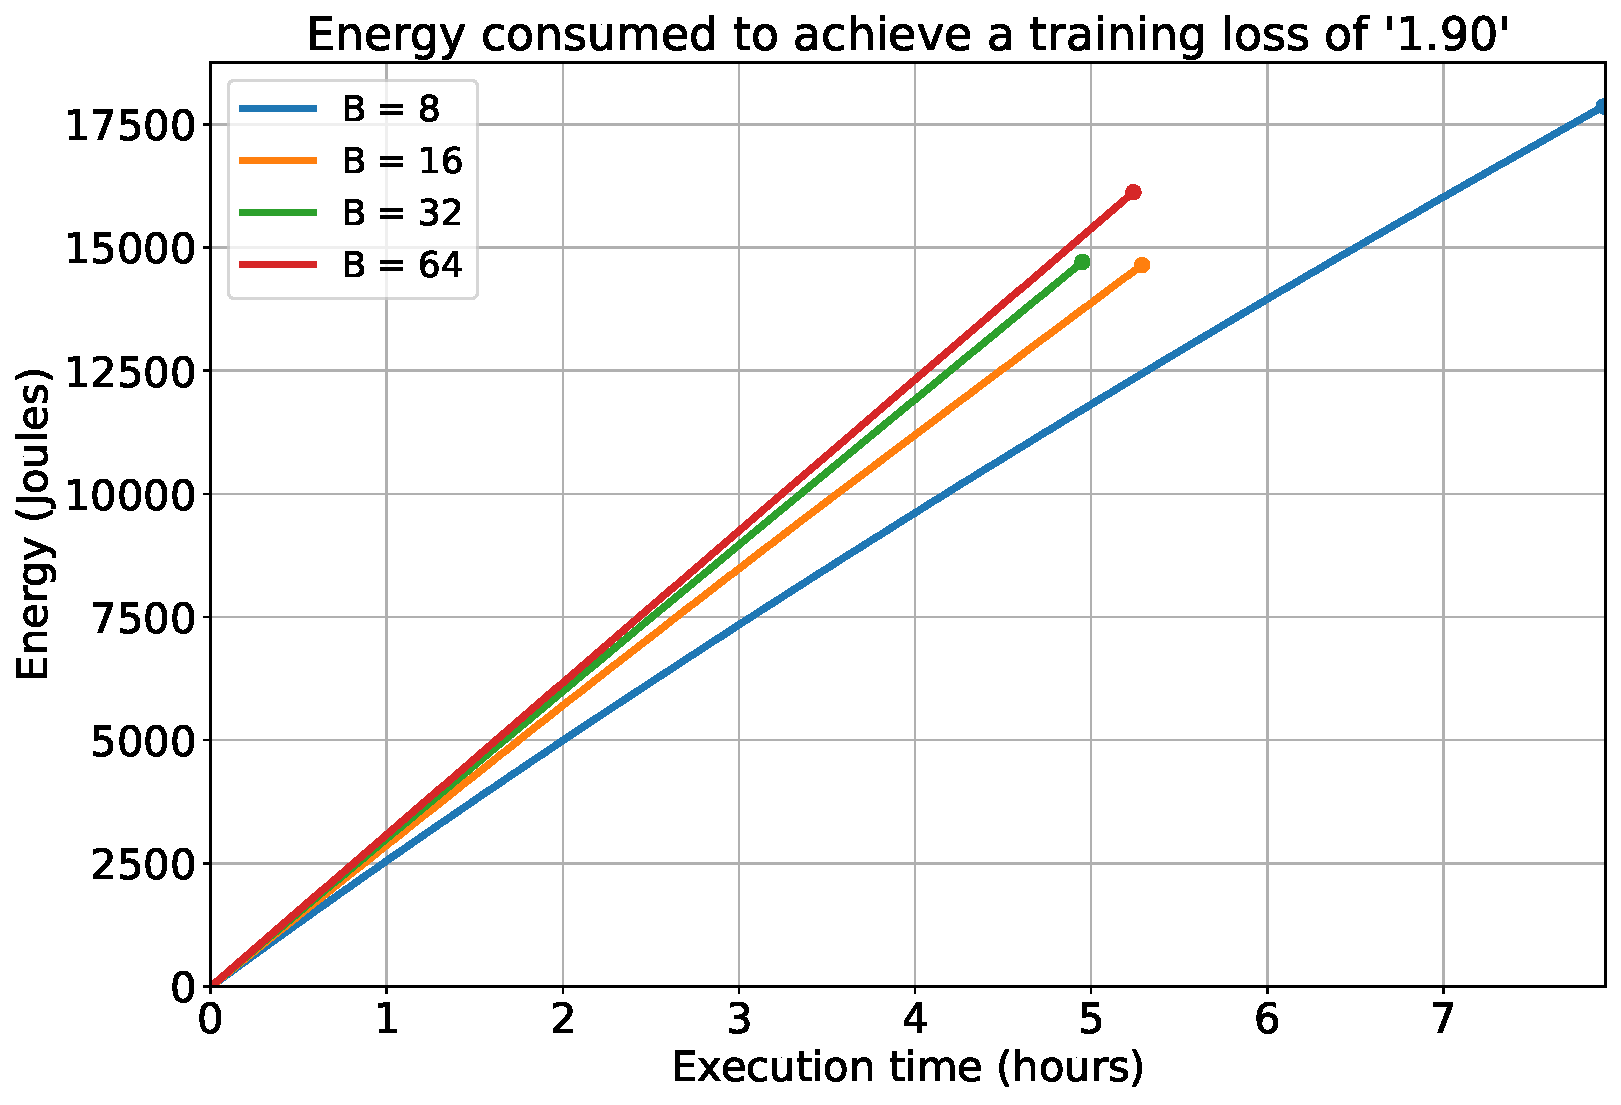
\includegraphics[trim = {0.0in 0.0in 0.0in 0.0in}, clip, width = 1.0 \textwidth]{../Figures/time_vs_energy_converged_training_190.pdf}
                \caption{Energy for converging to training loss of $1.9$}
                \label{fig:convergence_energy_training_190}
            \end{subfigure}
            \caption{Energy measurements for prespecified accuracy thresholds based on the training loss}
            \label{fig:convergence_threshold_training}
        \end{figure}

        General wisdom suggests to train AI jobs with the largest batch size possible to improve convergence and resource utilization. This assumption comes at the cost of higher energy consumption as the cost-per-iteration is higher due to the increased computational load. However, as we can observe from Figure~\ref{fig:convergence_threshold_training}, it possible to achieve the same levels of accuracy with smaller batch sizes while minimizing the energy consumption. Moreover, general wisdom dictates as well that using a larger batch size could lead to faster execution times as the model converges faster. From the results shown we see that, not only is it energy wasteful to use larger batch sizes, but it can also slow down the training. Our results show it took more time to converge to the desired accuracy for the $B = 64$ results when compared to $B = 16$ and $B = 32$ for threshold 2.1, and $B = 16$ for threshold 1.9. Figure~\ref{fig:accuracy_vs_time_and_energy_training} presents the total time and energy spent for a range of accuracy thresholds. These plots are meant to guide decision choices in terms of what batch size to use for a given threshold so that execution time or energy consumption are minimized. For a desired training loss, these plots can be used to find what batch size gives the best execution time and/or best energy consumption.

        \begin{figure}[!t]
            \centering
            \begin{subfigure}[b]{0.47 \textwidth}
                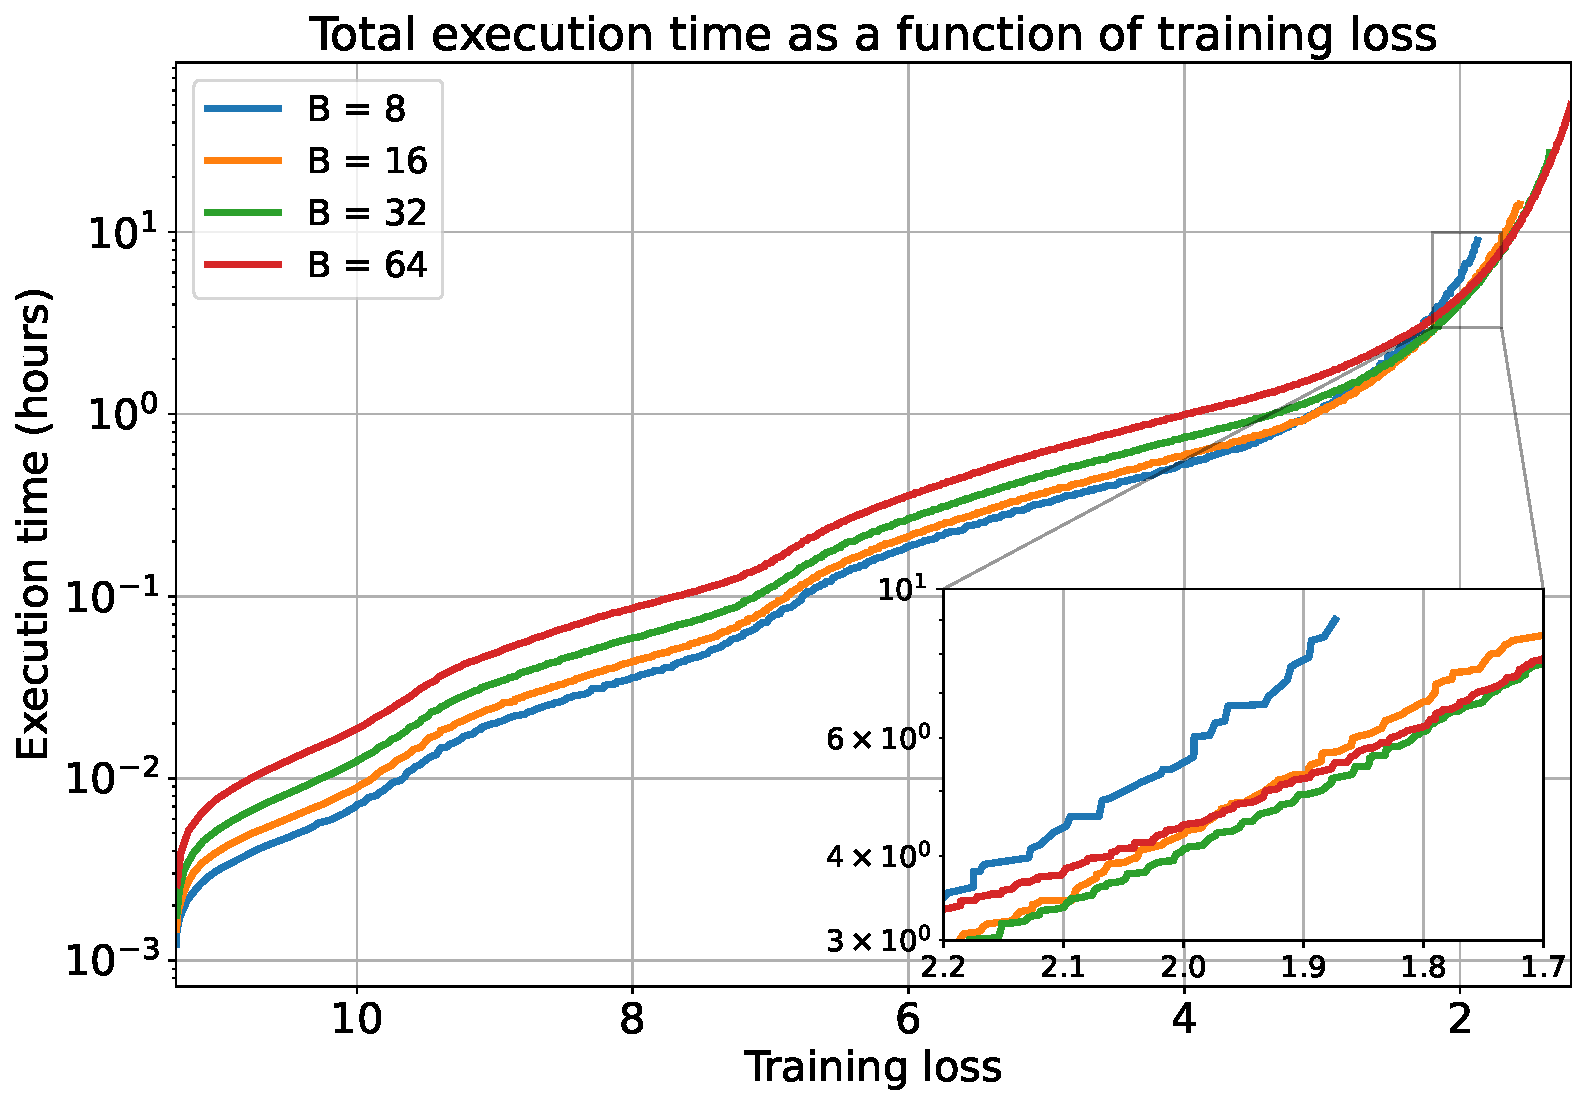
\includegraphics[trim = {0.0in 0.00in 0.0in 0.0in}, clip, width = 1.02 \textwidth]{../Figures/accuracy_vs_time_training.pdf}
                \caption{Execution time as a functions of the training loss}
                \label{fig:accuracy_vs_time_training}
            \end{subfigure}
            ~
            \begin{subfigure}[b]{0.47 \textwidth}
                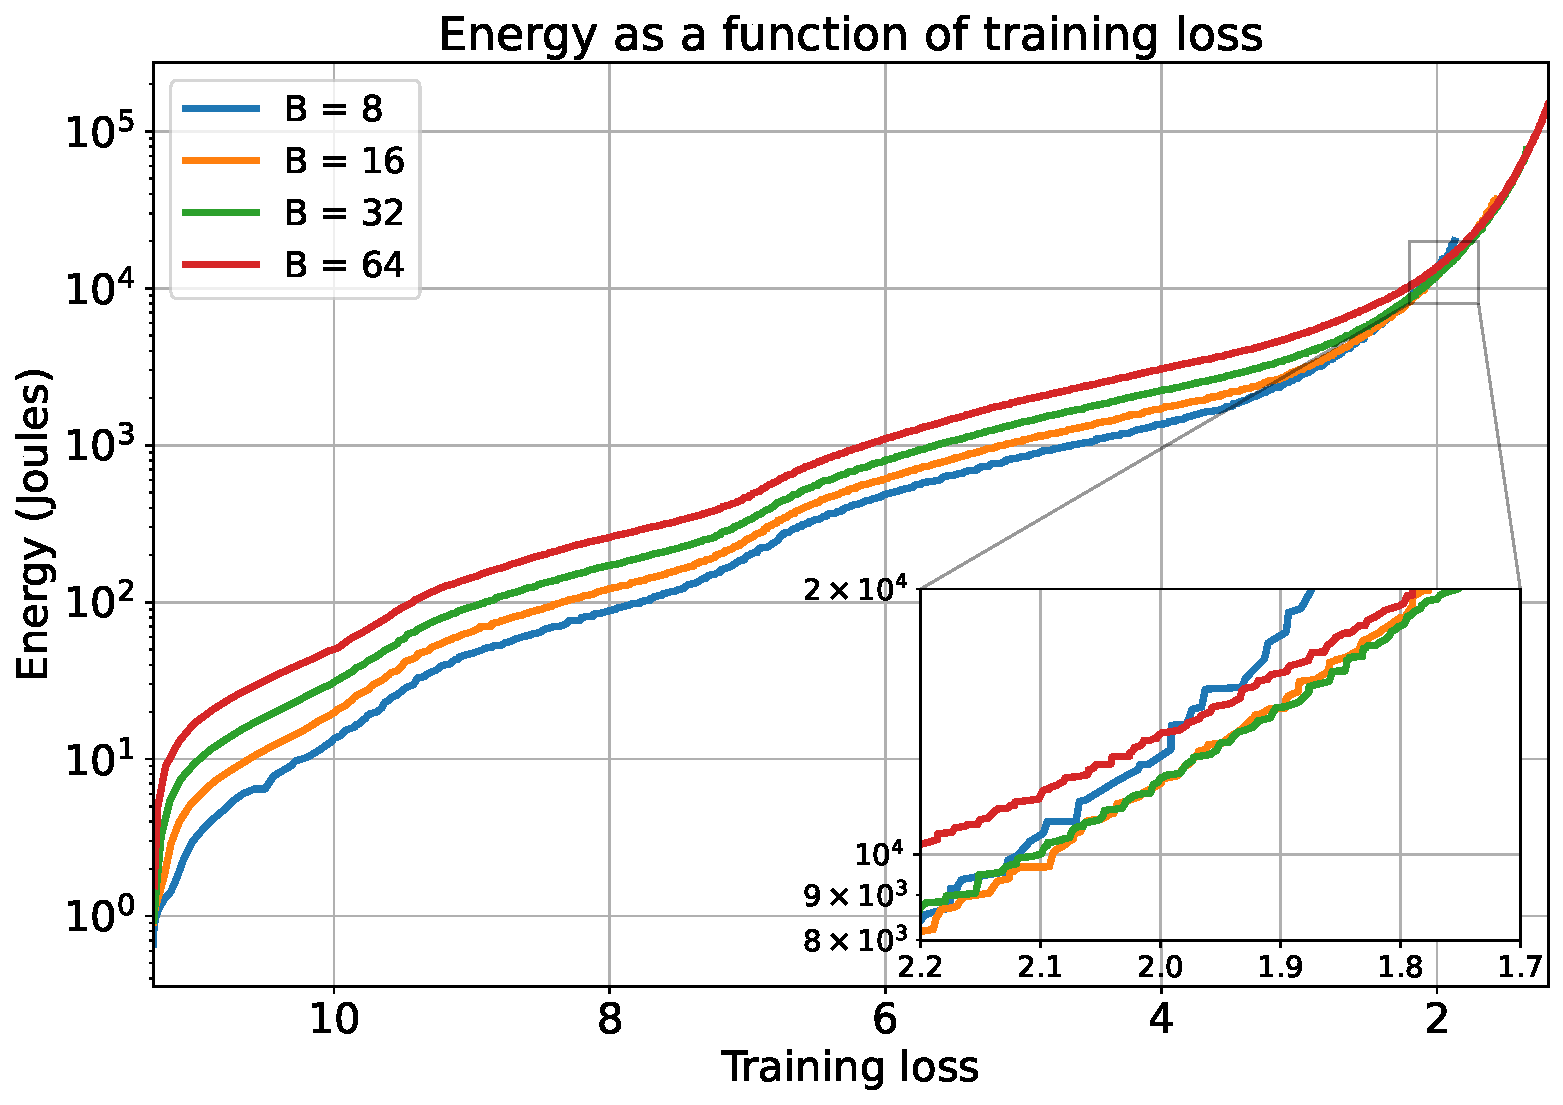
\includegraphics[trim = {0.0in 0.0in 0.0in 0.0in}, clip, width = 1.0 \textwidth]{../Figures/accuracy_vs_energy_training.pdf}
                \caption{Energy as a functions of the training loss}
                \label{fig:accuracy_vs_energy_training}
            \end{subfigure}
            \caption{Execution time and energy measurements for a range of accuracy thresholds based on the training loss}
            \label{fig:accuracy_vs_time_and_energy_training}
        \end{figure}
    }

    \section{Conclusions and Future Work}
    {
        Training and deploying FM tools has become the target of machine learning as incredible results have been achieved with the potential to be improved as larger and larger models are trained. However, it is important to enable this technology in a sustainable way through efficient resource utilization and minimizing energy waste. This study aims to provide guidelines to ML engineers to help them choose how to approach a training job with sustainability metrics in mind, as opposed to just focusing purely on the model accuracy. We saw that, common wisdom may not apply if energy is to be considered as saturating the GPU devices is not necessarily the most efficient way to run a training job. To fully understand the impact of GPU saturation and hyperparameter choices in a more comprehensive way, more studies with different models need to be performed. Furthermore, exploiting hardware constraints such as GPU frequency, can compensate for the increase in computational cost while preserving the model convergence and thus it is another aspect of the training that we aim to look at in the future.
    }

    \clearpage

    \appendix

    \section{Accuracy in terms of validation loss}
    {
        In the results section, we present our analysis based on the \textit{training} loss. A more realistic metric is to use the \textit{validation} loss, which evaluates a partially trained model with a validation dataset for the purpose of understanding how well the training is performing. Contrary to the training loss, the validation loss is not provided to the training algorithm and is meant to provide a more ``realistic'' view of how well the model does in a real-world deployment. The following plots are the same as the ones before with the validation loss used as the accuracy metric.

        \begin{figure}[!h]
            \centering
            \captionsetup[subfigure]{margin = {0.0in,0.0in}}
            \begin{subfigure}[b]{0.47 \textwidth}
                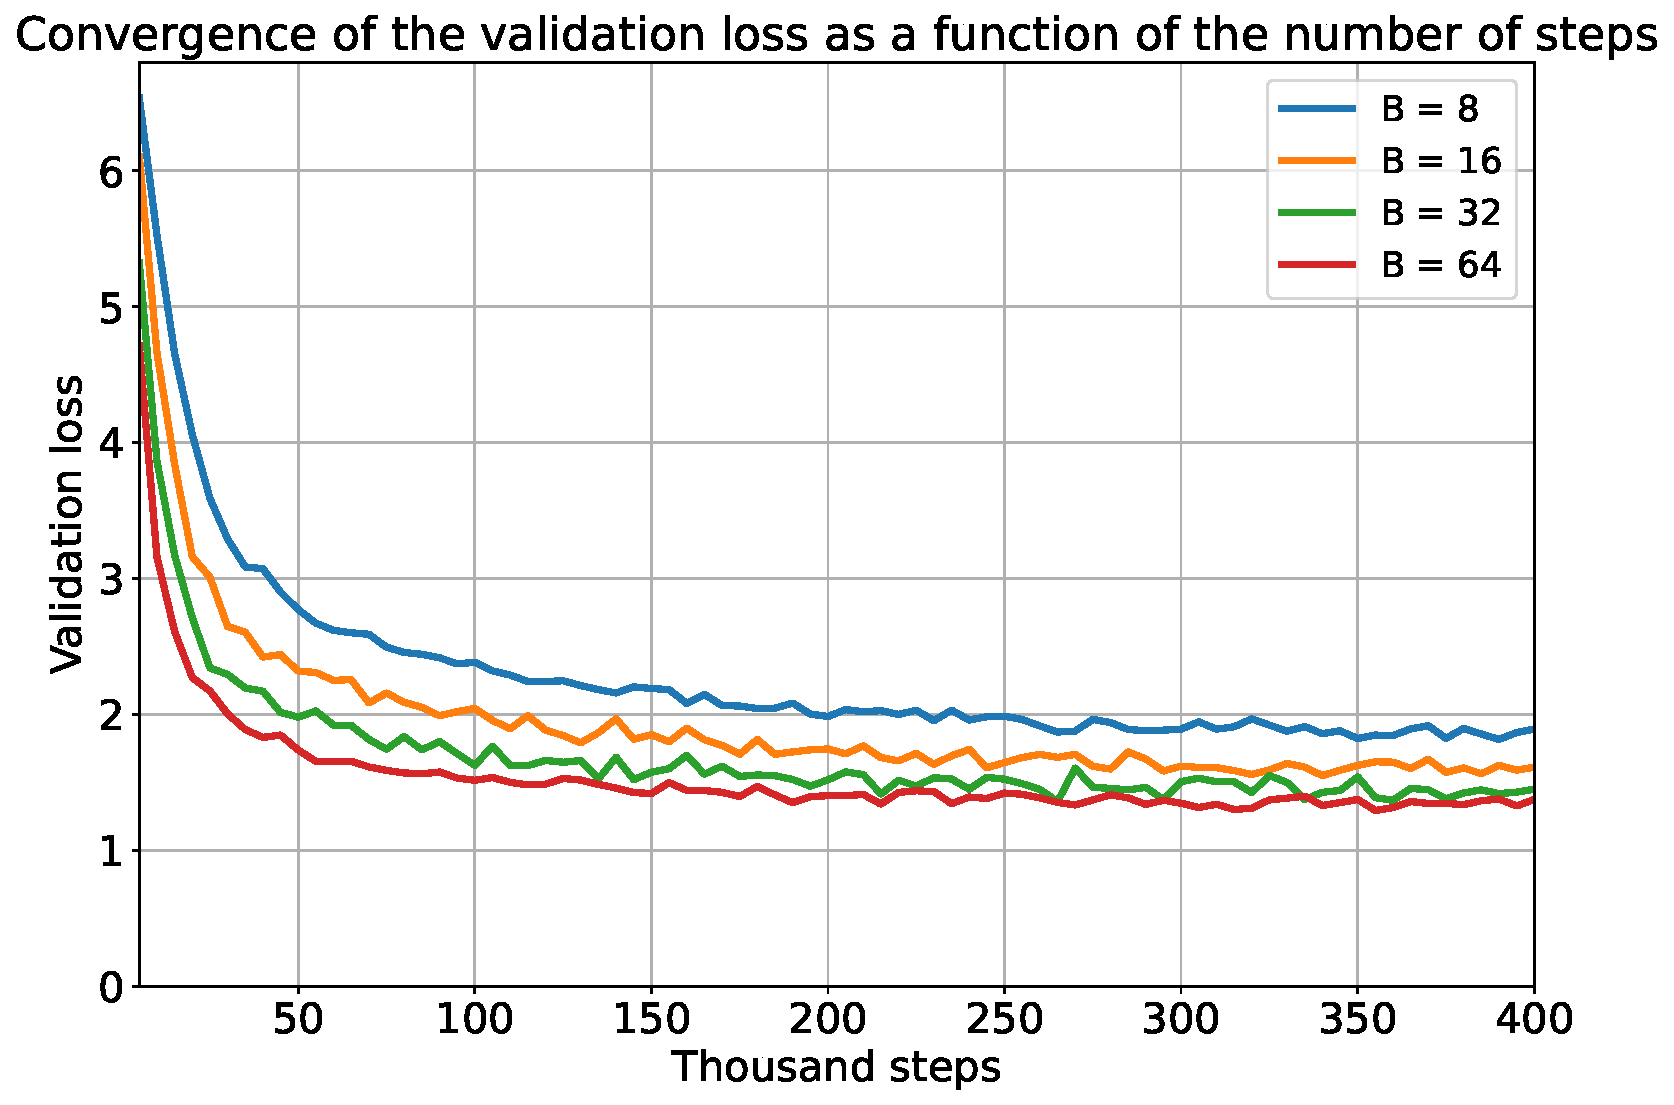
\includegraphics[trim = {0.0in 0.0in 0.0in 0.0in}, clip, width = 1.0 \textwidth]{../Figures/convergence_history_validation.pdf}
                \caption{Convergence as a function of the number of steps}
                \label{fig:convergence_accuracy_validation}
            \end{subfigure}
            ~
            \captionsetup[subfigure]{margin = {0.2in,0.0in}}
            \begin{subfigure}[b]{0.47 \textwidth}
                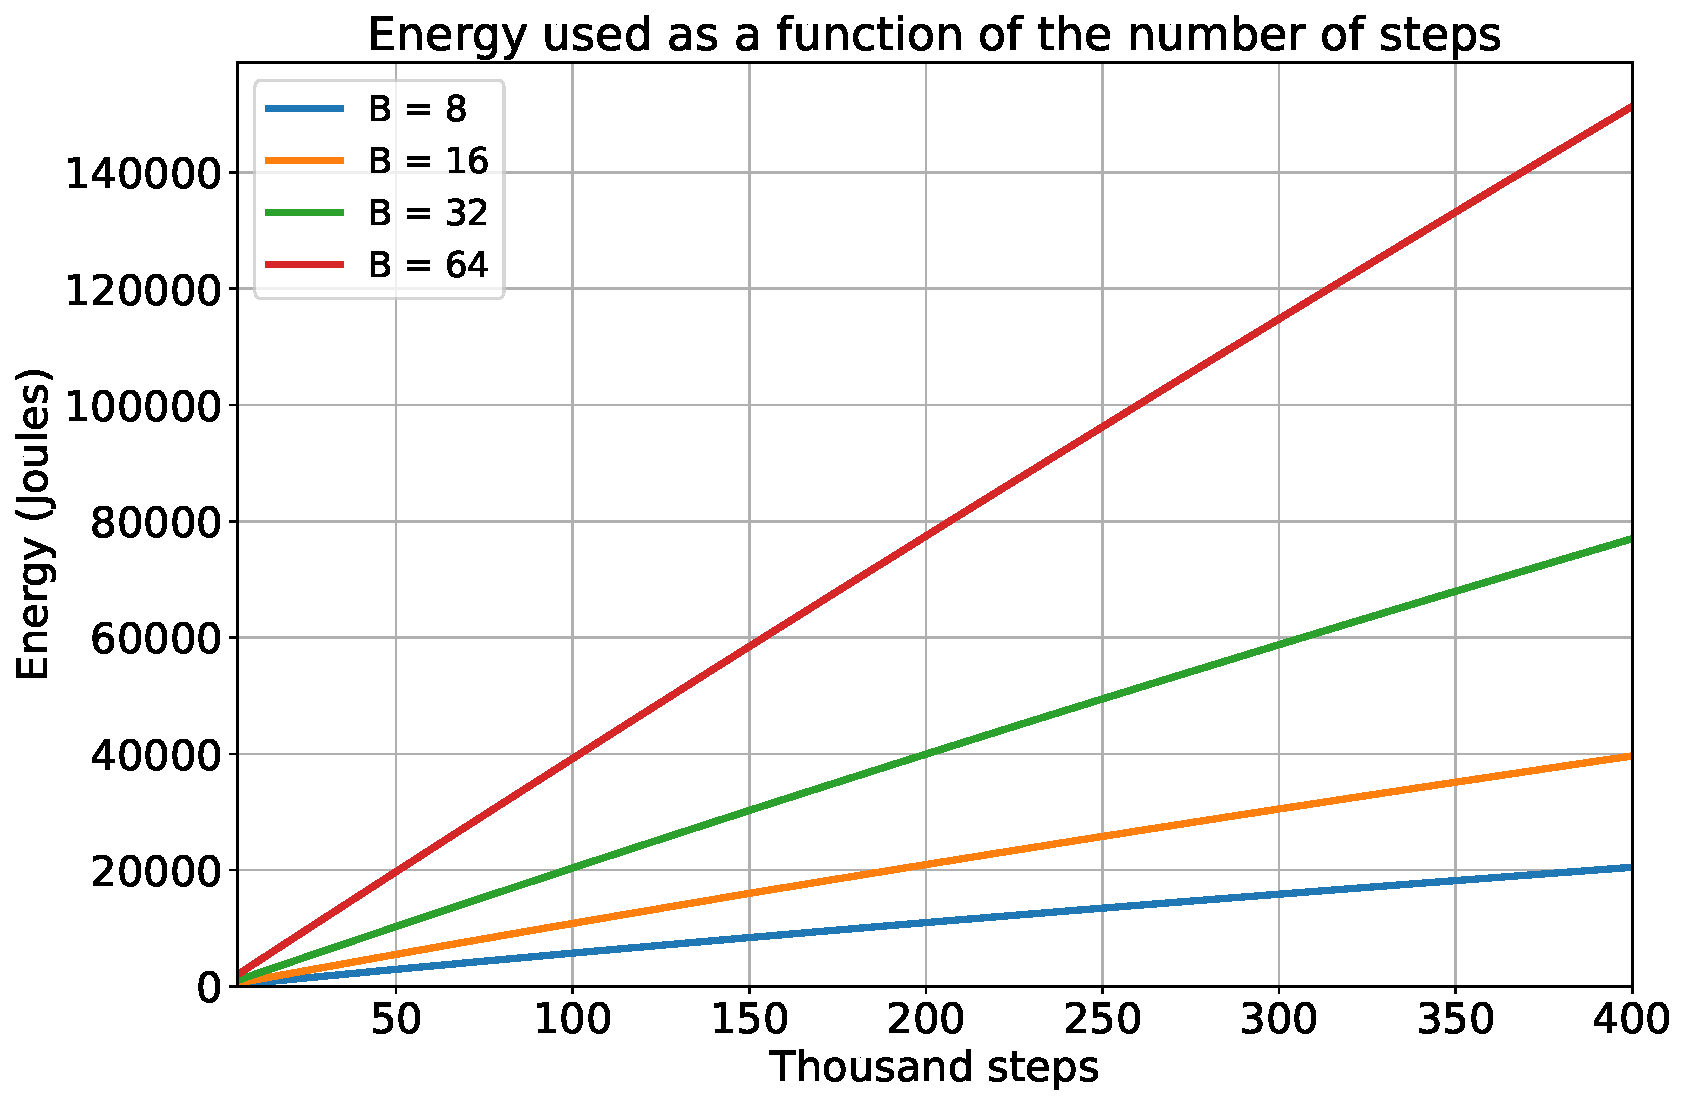
\includegraphics[trim = {0.0in 0.01in 0.0in 0.0in}, clip, width = 1.005 \textwidth]{../Figures/energy_history_validation.pdf}
                \caption{Energy used as a function of the number of steps}
                \label{fig:convergence_energy_validation}
            \end{subfigure}
            ~
            \captionsetup[subfigure]{margin = {0.0in,0.0in}}
            \begin{subfigure}[b]{0.47 \textwidth}
                \vspace{1.0em}
                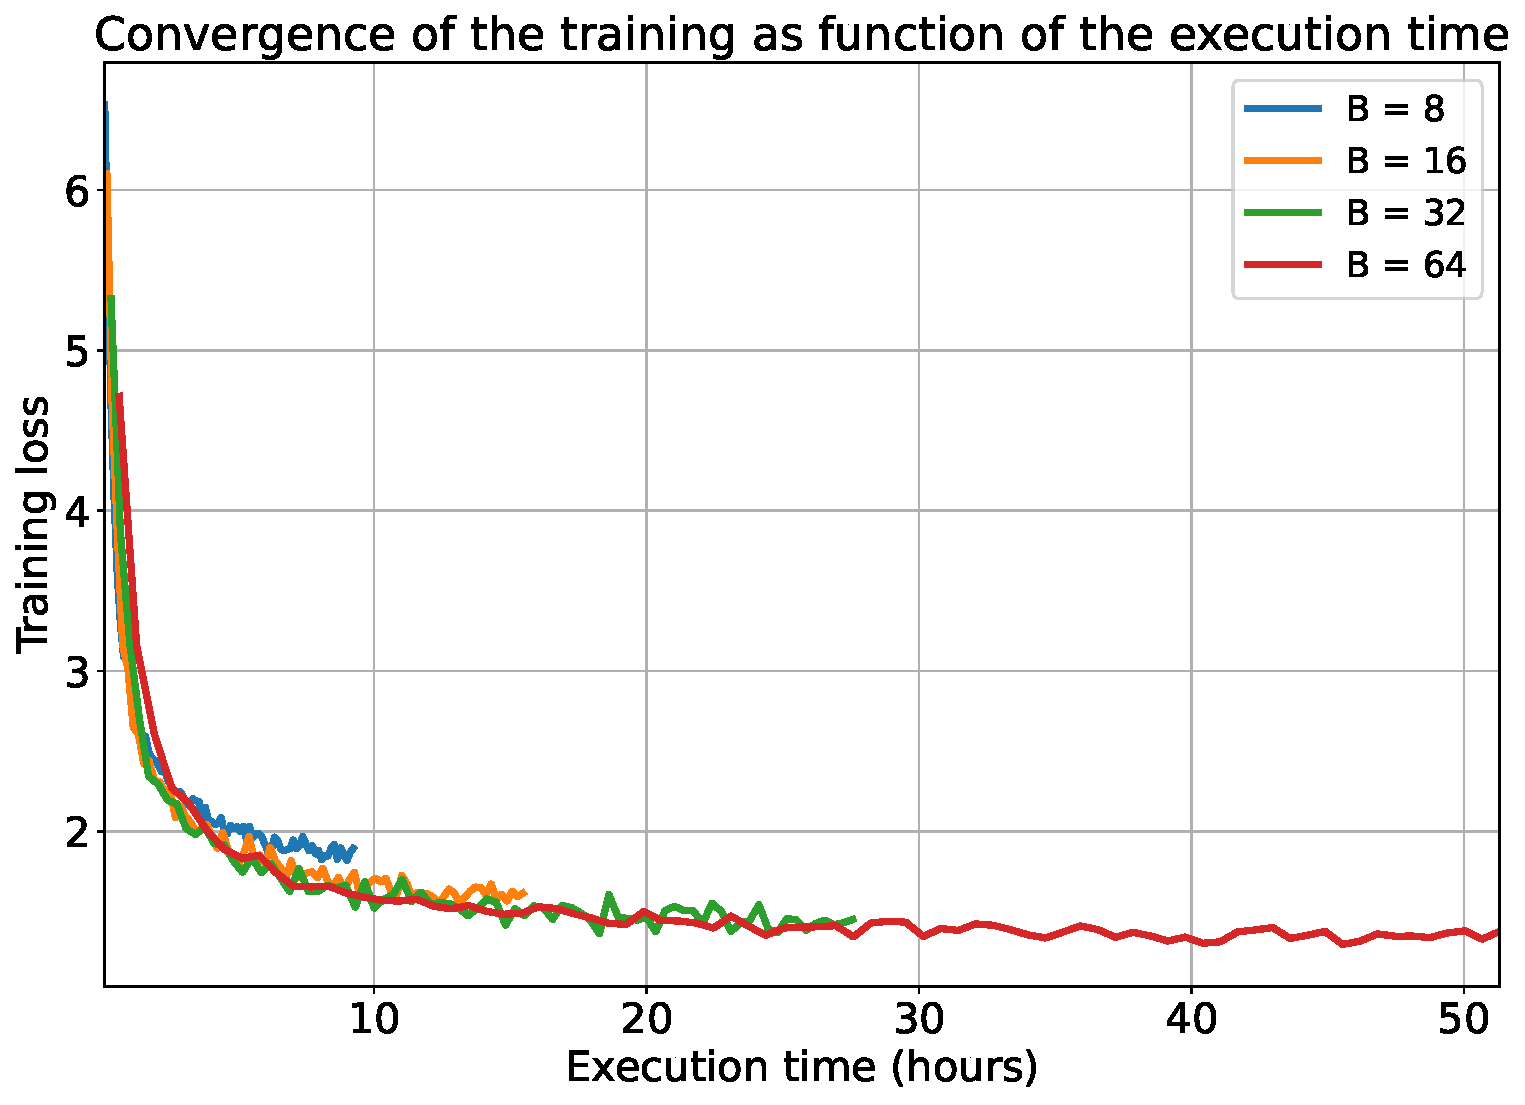
\includegraphics[trim = {0.0in 0.0in 0.0in 0.0in}, clip, width = 1.0 \textwidth]{../Figures/time_vs_accuracy_validation.pdf}
                \caption{Convergence as a function of the execution time}
                \label{fig:time_vs_accuracy_validation}
            \end{subfigure}
            ~
            \captionsetup[subfigure]{margin = {0.2in,0.0in}}
            \begin{subfigure}[b]{0.47 \textwidth}
                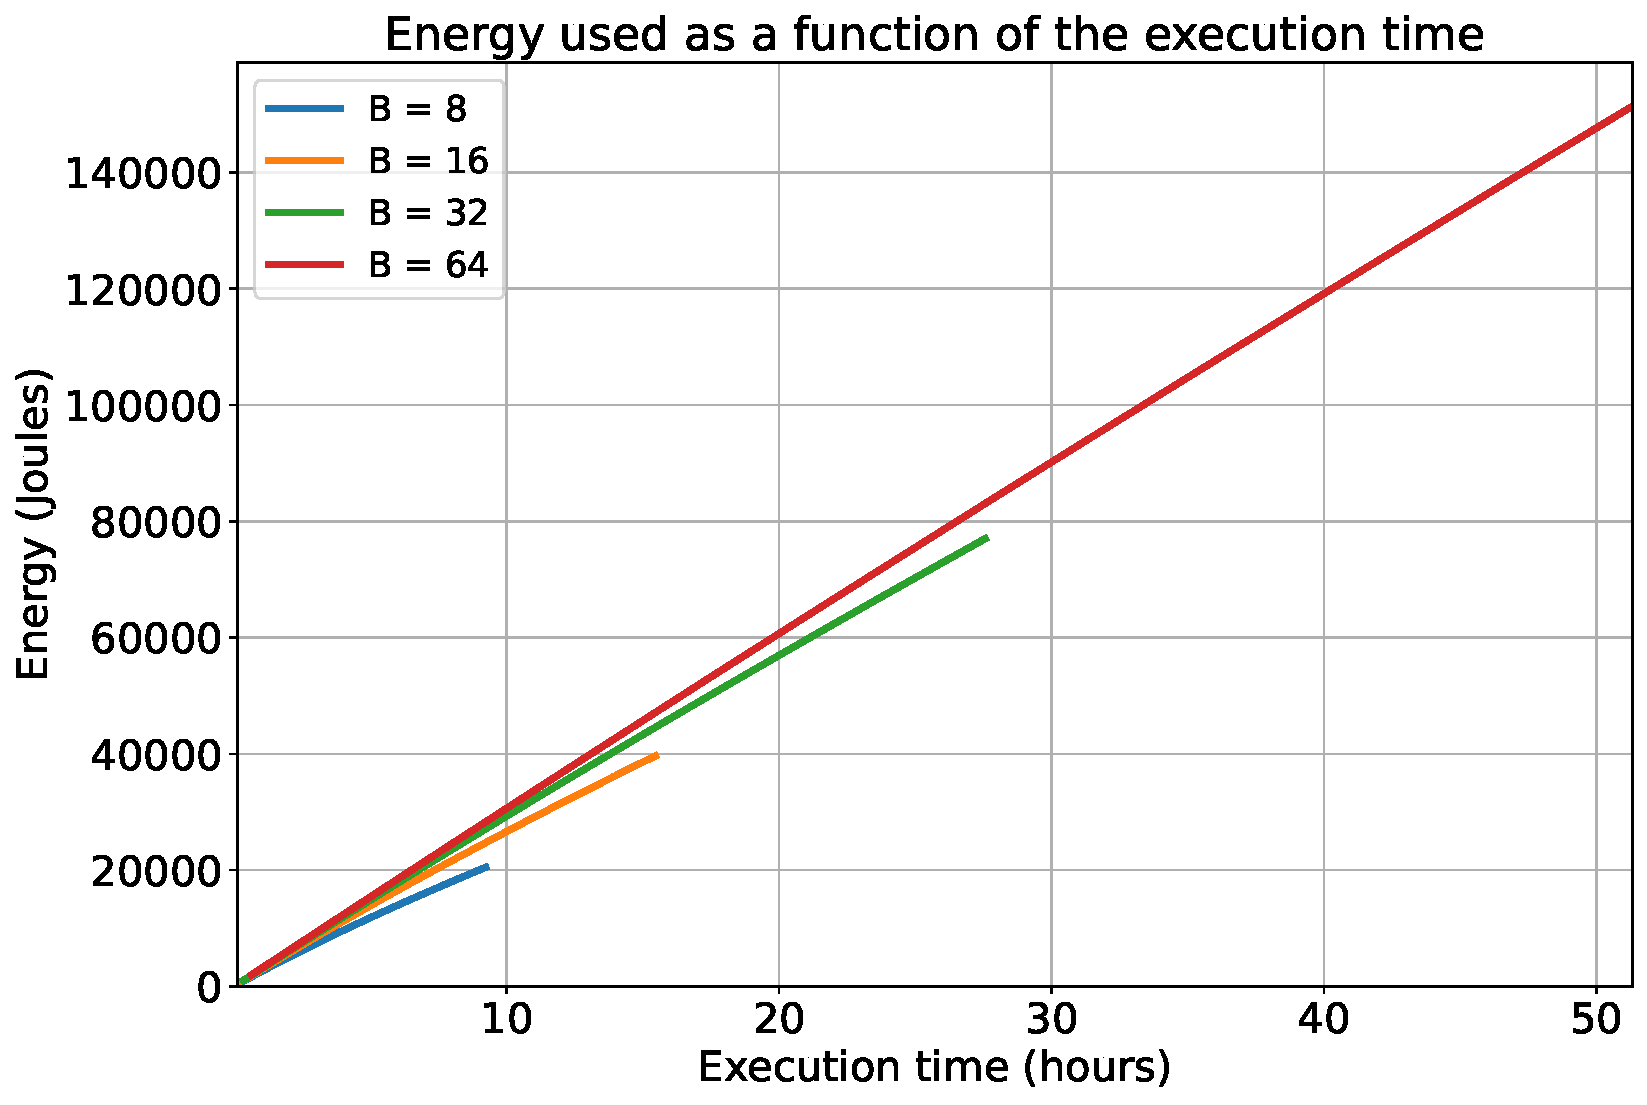
\includegraphics[trim = {0.0in 0.01in 0.0in 0.0in}, clip, width = 1.085 \textwidth]{../Figures/time_vs_energy_validation.pdf}
                \caption{Energy used as a function of the execution time}
                \label{fig:time_vs_energy_validation}
            \end{subfigure}
            \caption{Convergence and energy measurements over the complete unstopped execution (i.e., all $N = 400000$ training steps)}
            \label{fig:unstopped_execution_validation}
        \end{figure}

        \clearpage

        \begin{figure}[H]
            \centering
            \captionsetup[subfigure]{margin = {0.2in,0.0in}}
            \begin{subfigure}[b]{0.47 \textwidth}
                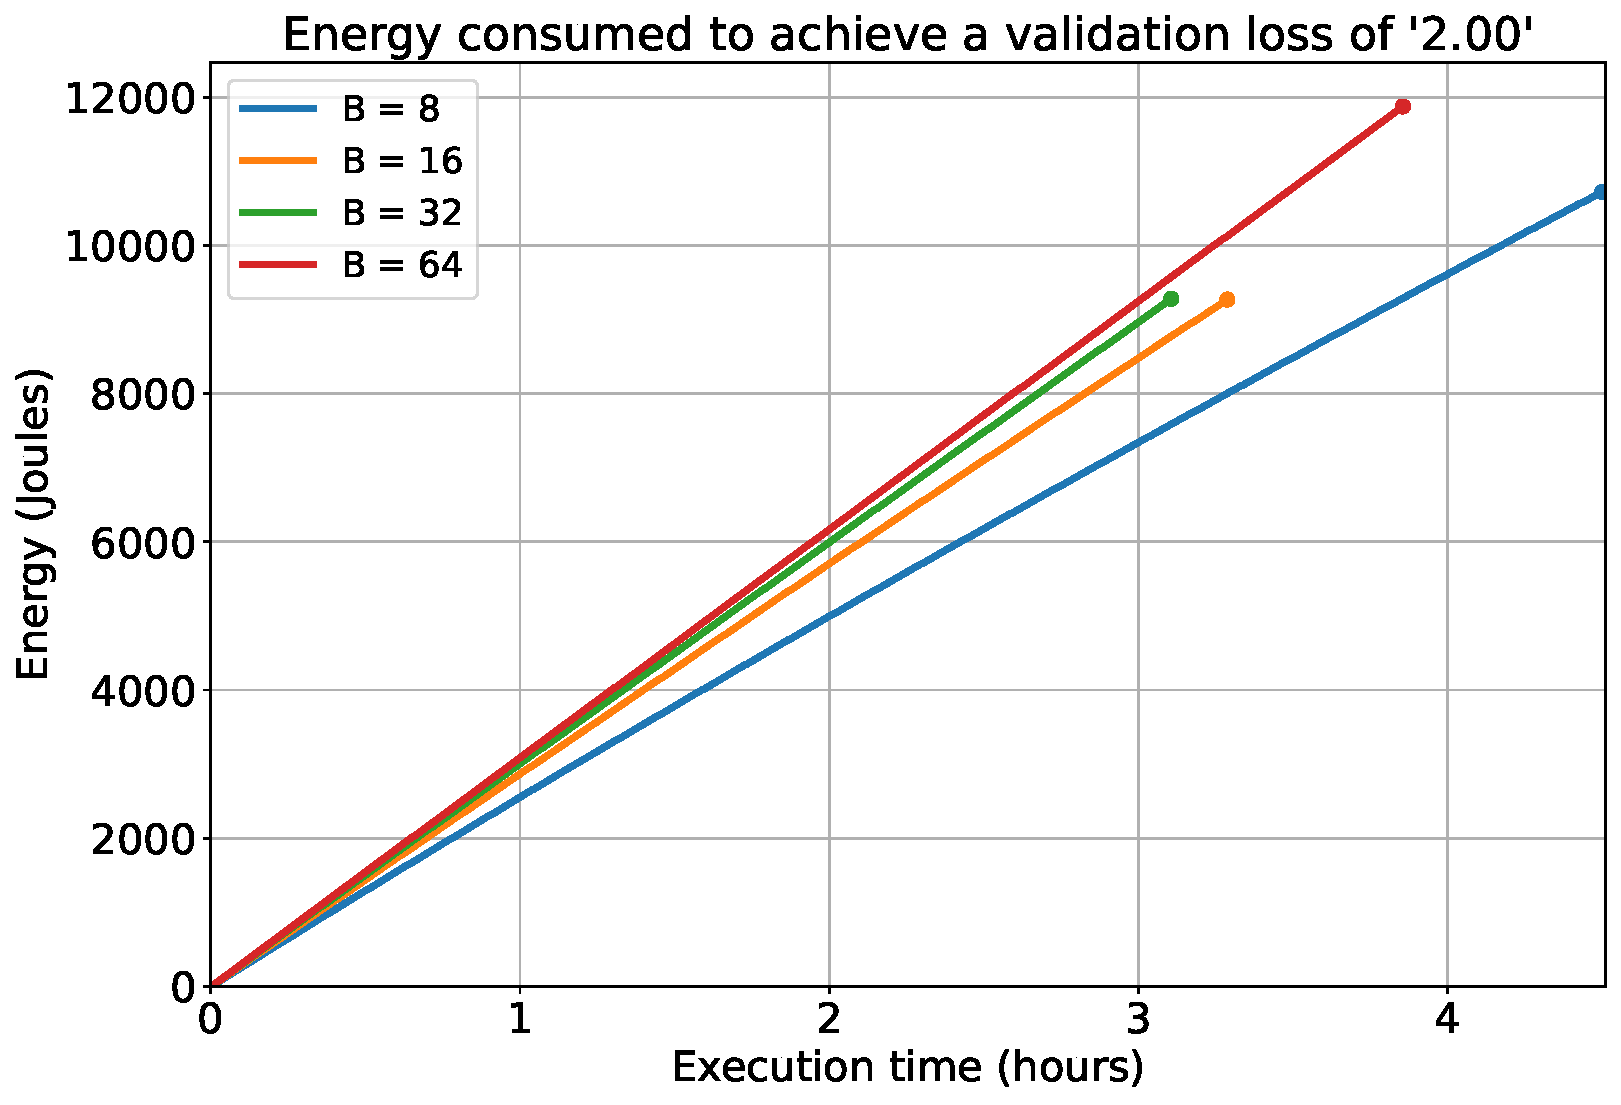
\includegraphics[trim = {0.0in 0.0in 0.0in 0.0in}, clip, width = 1.0 \textwidth]{../Figures/time_vs_energy_converged_validation_200.pdf}
                \caption{Energy for converging to validation loss of $2.1$}
                \label{fig:convergence_energy_validation_200}
            \end{subfigure}
            ~
            \captionsetup[subfigure]{margin = {0.2in,0.0in}}
            \begin{subfigure}[b]{0.47 \textwidth}
                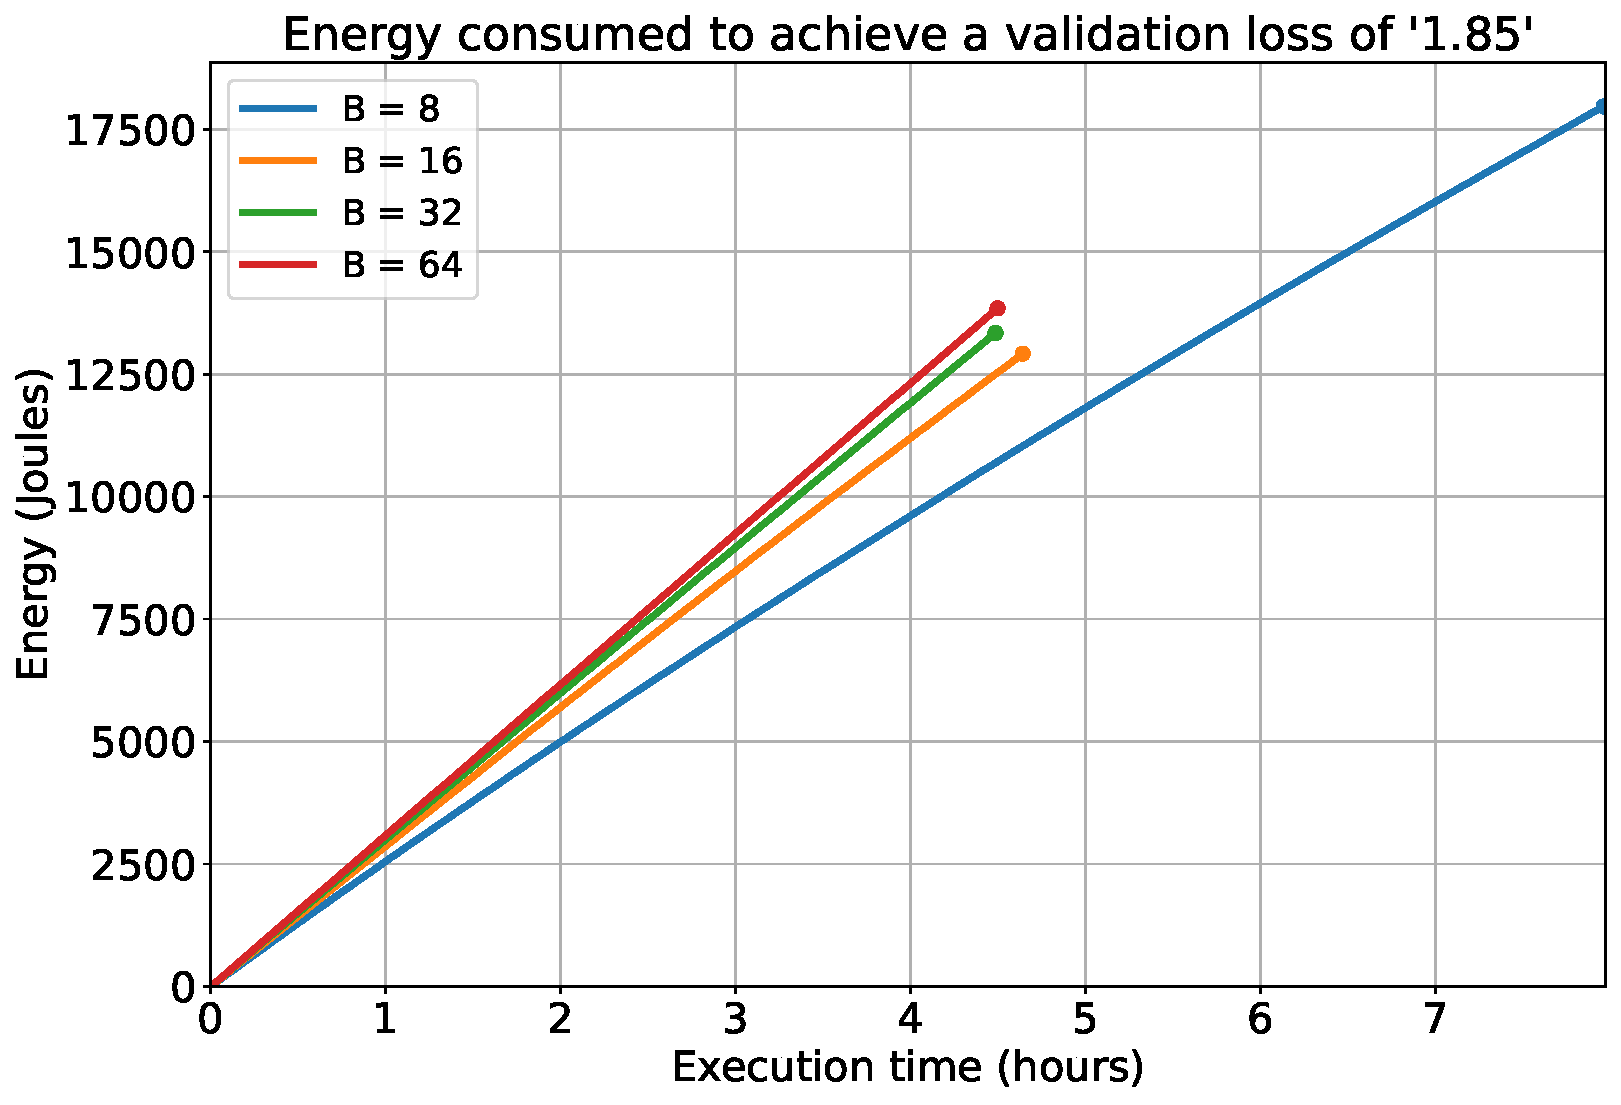
\includegraphics[trim = {0.0in 0.0in 0.0in 0.0in}, clip, width = 1.0 \textwidth]{../Figures/time_vs_energy_converged_validation_185.pdf}
                \caption{Energy for converging to validation loss of $1.85$}
                \label{fig:convergence_energy_validation_185}
            \end{subfigure}
            \caption{Energy measurements for prespecified accuracy thresholds based on the validation loss}
            \label{fig:time_vs_energy_validation}
        \end{figure}

        \begin{figure}[H]
            \centering
            \begin{subfigure}[b]{0.47 \textwidth}
                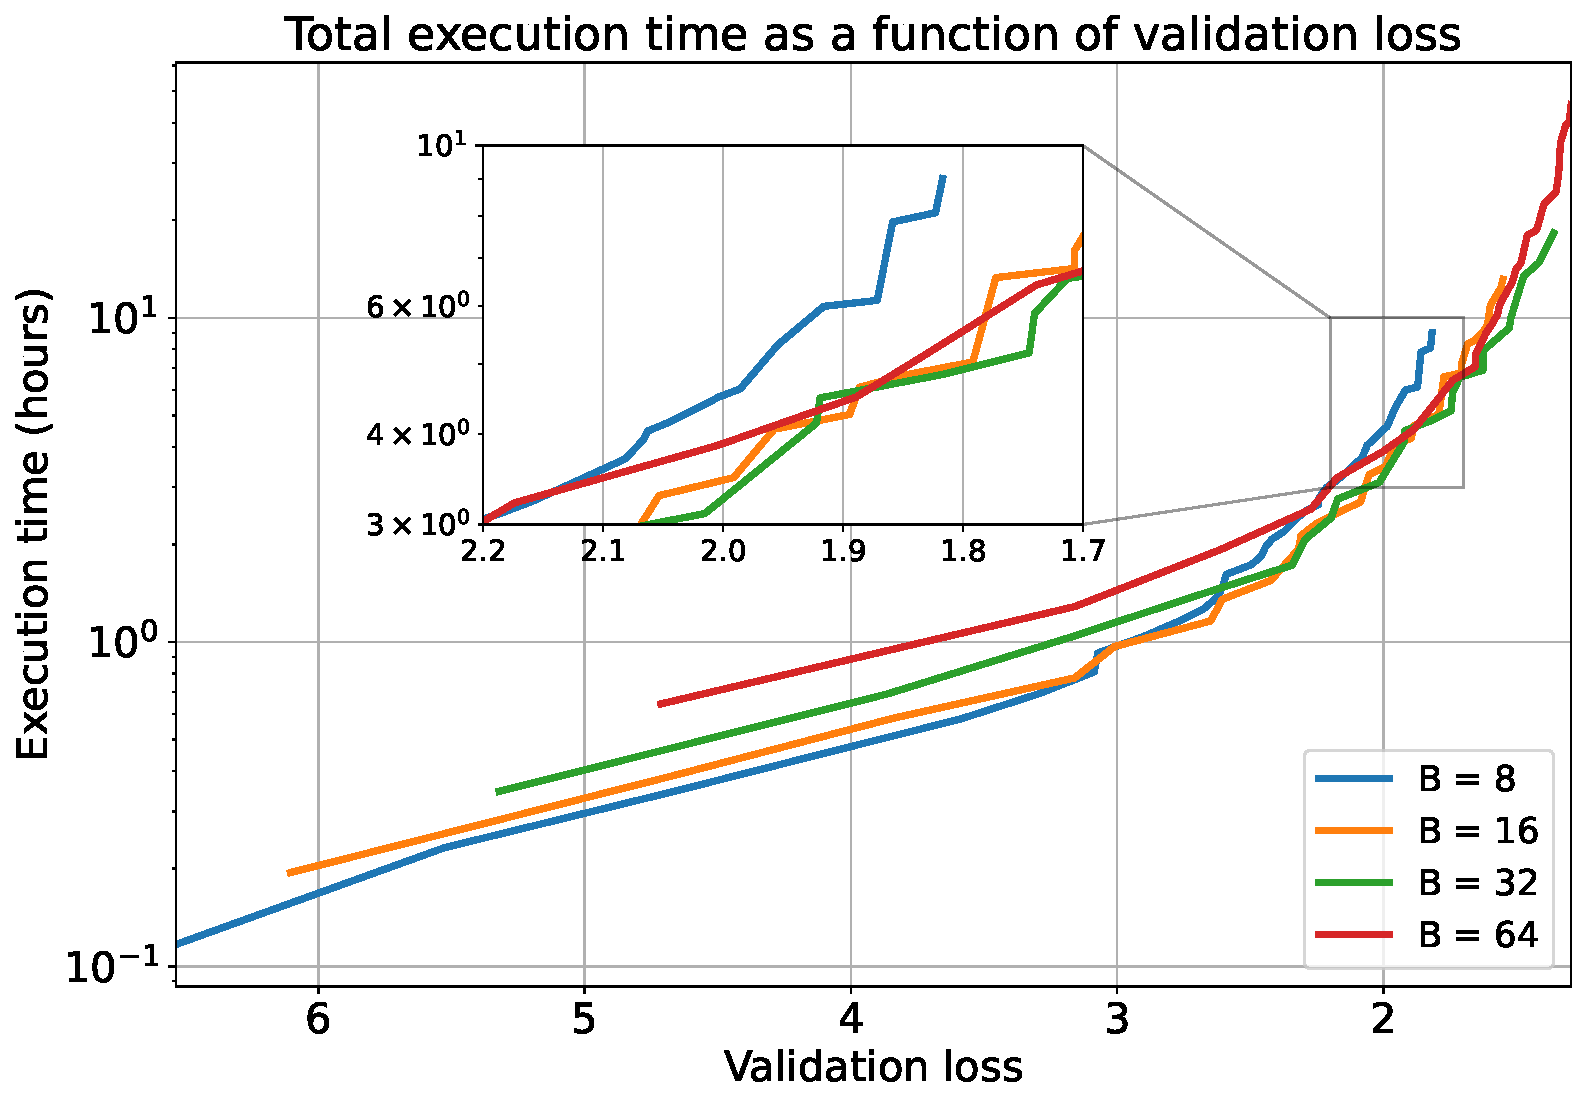
\includegraphics[trim = {0.0in 0.00in 0.0in 0.0in}, clip, width = 1.02 \textwidth]{../Figures/accuracy_vs_time_validation.pdf}
                \caption{Execution time as a functions of the validation loss}
                \label{fig:convergence_energy_validation}
            \end{subfigure}
            ~
            \begin{subfigure}[b]{0.47 \textwidth}
                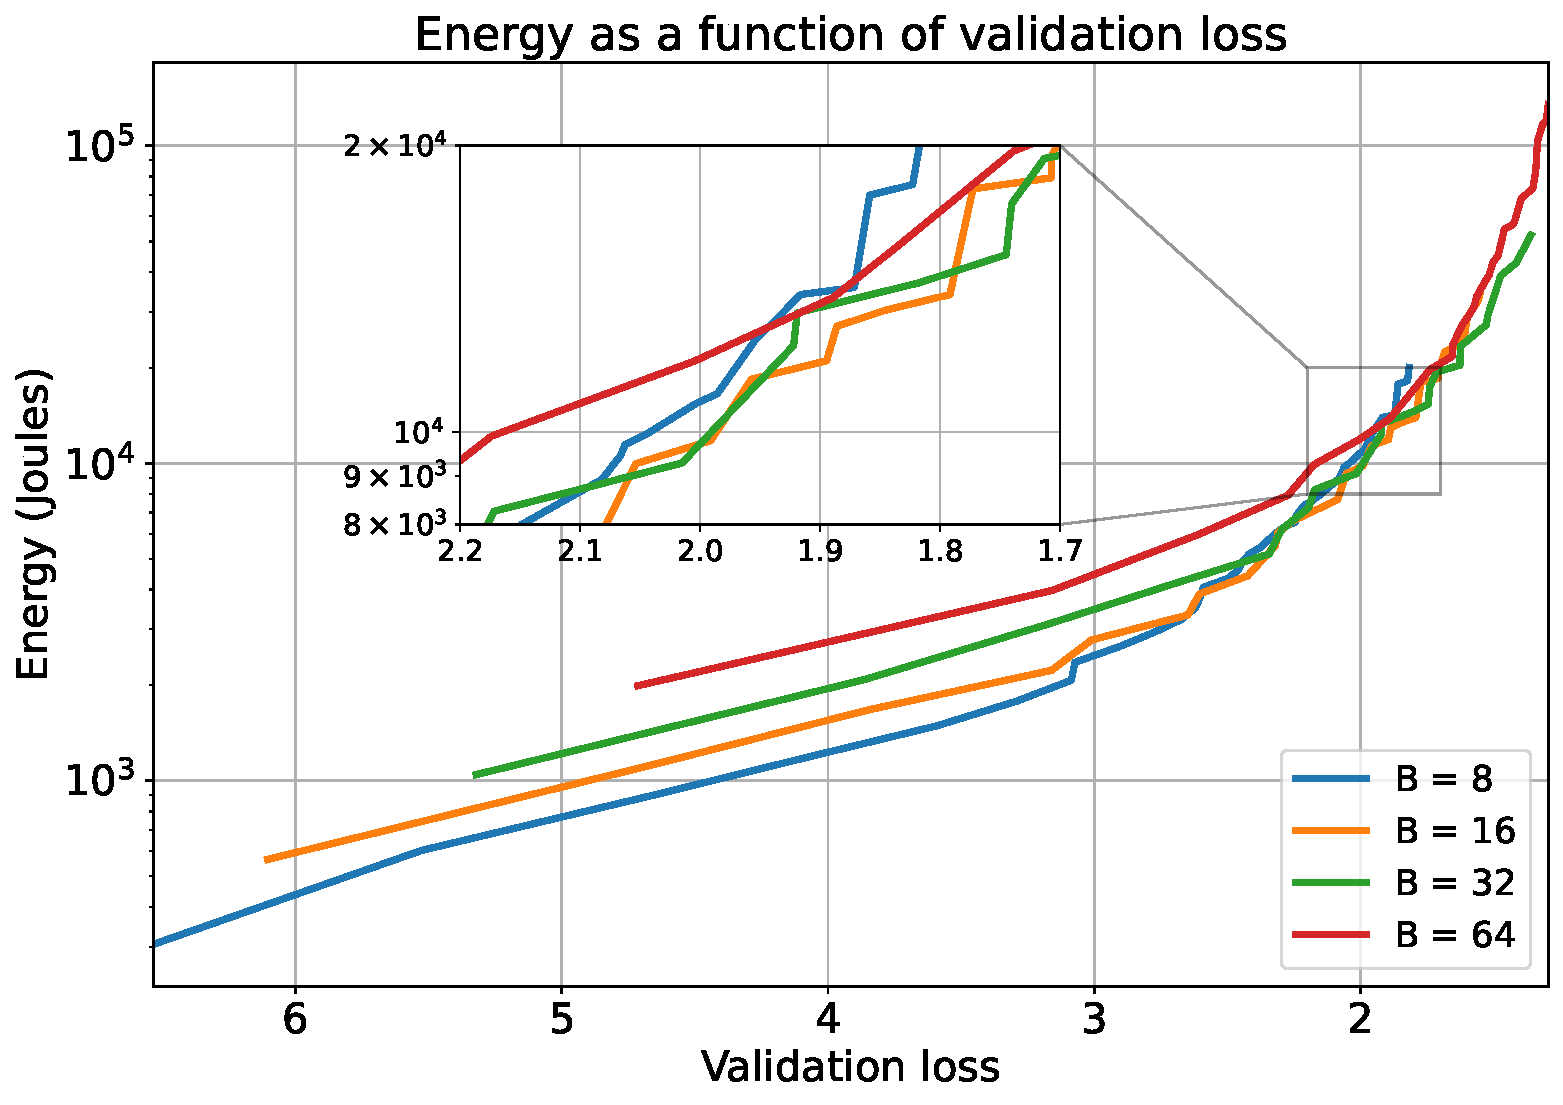
\includegraphics[trim = {0.0in 0.0in 0.0in 0.0in}, clip, width = 1.0 \textwidth]{../Figures/accuracy_vs_energy_validation.pdf}
                \caption{Energy as a functions of the validation loss}
                \label{fig:convergence_energy_validation}
            \end{subfigure}
            \caption{Execution time and energy measurements for a range of accuracy thresholds based on the validation loss}
            \label{fig:accuracy_vs_energy_validation}
        \end{figure}
    }
\end{document}
